\documentclass[aspectratio=169]{beamer}

% Shared preamble for Claude Code slide decks
% Usage: % Shared preamble for Claude Code slide decks
% Usage: % Shared preamble for Claude Code slide decks
% Usage: \input{preamble} after \documentclass[aspectratio=169]{beamer}

\usetheme{default}
\usecolortheme{dove}

\setbeamertemplate{navigation symbols}{}
\setbeamertemplate{footline}{%
  \hfill{\large\insertframenumber\,/\,\inserttotalframenumber}\hspace{0.8em}\vspace{0.5em}%
}

\definecolor{popblue}{RGB}{52, 101, 164}
\definecolor{sampred}{RGB}{204, 0, 0}
\definecolor{paramgreen}{RGB}{0, 140, 70}
\definecolor{lightbg}{RGB}{245, 245, 250}
\definecolor{warnred}{RGB}{180, 40, 40}
\definecolor{orange1}{RGB}{220, 120, 0}
\definecolor{violet1}{RGB}{120, 50, 160}

\setbeamercolor{frametitle}{fg=popblue}
\setbeamercolor{title}{fg=popblue}
\setbeamercolor{block title}{fg=white,bg=popblue}
\setbeamercolor{block body}{bg=lightbg}
\setbeamercolor{block title alerted}{fg=white,bg=warnred}
\setbeamercolor{block body alerted}{bg=lightbg}
\setbeamercolor{block title example}{fg=white,bg=paramgreen}
\setbeamercolor{block body example}{bg=lightbg}

\usepackage{listings}
\usepackage[T1]{fontenc}
\usepackage{hyperref}
\usepackage{tikz}
\usepackage{booktabs}
\usetikzlibrary{shapes, arrows.meta, positioning, calc}

\lstset{
  basicstyle=\ttfamily\scriptsize,
  keywordstyle=\color{popblue}\bfseries,
  stringstyle=\color{paramgreen},
  commentstyle=\color{gray},
  breaklines=true,
  frame=single,
  backgroundcolor=\color{lightbg},
  rulecolor=\color{popblue!30},
  showstringspaces=false,
  columns=fullflexible,
}
 after \documentclass[aspectratio=169]{beamer}

\usetheme{default}
\usecolortheme{dove}

\setbeamertemplate{navigation symbols}{}
\setbeamertemplate{footline}{%
  \hfill{\large\insertframenumber\,/\,\inserttotalframenumber}\hspace{0.8em}\vspace{0.5em}%
}

\definecolor{popblue}{RGB}{52, 101, 164}
\definecolor{sampred}{RGB}{204, 0, 0}
\definecolor{paramgreen}{RGB}{0, 140, 70}
\definecolor{lightbg}{RGB}{245, 245, 250}
\definecolor{warnred}{RGB}{180, 40, 40}
\definecolor{orange1}{RGB}{220, 120, 0}
\definecolor{violet1}{RGB}{120, 50, 160}

\setbeamercolor{frametitle}{fg=popblue}
\setbeamercolor{title}{fg=popblue}
\setbeamercolor{block title}{fg=white,bg=popblue}
\setbeamercolor{block body}{bg=lightbg}
\setbeamercolor{block title alerted}{fg=white,bg=warnred}
\setbeamercolor{block body alerted}{bg=lightbg}
\setbeamercolor{block title example}{fg=white,bg=paramgreen}
\setbeamercolor{block body example}{bg=lightbg}

\usepackage{listings}
\usepackage[T1]{fontenc}
\usepackage{hyperref}
\usepackage{tikz}
\usepackage{booktabs}
\usetikzlibrary{shapes, arrows.meta, positioning, calc}

\lstset{
  basicstyle=\ttfamily\scriptsize,
  keywordstyle=\color{popblue}\bfseries,
  stringstyle=\color{paramgreen},
  commentstyle=\color{gray},
  breaklines=true,
  frame=single,
  backgroundcolor=\color{lightbg},
  rulecolor=\color{popblue!30},
  showstringspaces=false,
  columns=fullflexible,
}
 after \documentclass[aspectratio=169]{beamer}

\usetheme{default}
\usecolortheme{dove}

\setbeamertemplate{navigation symbols}{}
\setbeamertemplate{footline}{%
  \hfill{\large\insertframenumber\,/\,\inserttotalframenumber}\hspace{0.8em}\vspace{0.5em}%
}

\definecolor{popblue}{RGB}{52, 101, 164}
\definecolor{sampred}{RGB}{204, 0, 0}
\definecolor{paramgreen}{RGB}{0, 140, 70}
\definecolor{lightbg}{RGB}{245, 245, 250}
\definecolor{warnred}{RGB}{180, 40, 40}
\definecolor{orange1}{RGB}{220, 120, 0}
\definecolor{violet1}{RGB}{120, 50, 160}

\setbeamercolor{frametitle}{fg=popblue}
\setbeamercolor{title}{fg=popblue}
\setbeamercolor{block title}{fg=white,bg=popblue}
\setbeamercolor{block body}{bg=lightbg}
\setbeamercolor{block title alerted}{fg=white,bg=warnred}
\setbeamercolor{block body alerted}{bg=lightbg}
\setbeamercolor{block title example}{fg=white,bg=paramgreen}
\setbeamercolor{block body example}{bg=lightbg}

\usepackage{listings}
\usepackage[T1]{fontenc}
\usepackage{hyperref}
\usepackage{tikz}
\usepackage{booktabs}
\usetikzlibrary{shapes, arrows.meta, positioning, calc}

\lstset{
  basicstyle=\ttfamily\scriptsize,
  keywordstyle=\color{popblue}\bfseries,
  stringstyle=\color{paramgreen},
  commentstyle=\color{gray},
  breaklines=true,
  frame=single,
  backgroundcolor=\color{lightbg},
  rulecolor=\color{popblue!30},
  showstringspaces=false,
  columns=fullflexible,
}


\title{Claude Code in Action}
\subtitle{Tool Use $\cdot$ Context $\cdot$ Hooks $\cdot$ MCP $\cdot$ SDK}
\date{}

\begin{document}

% ──────────────────────────────────────────────
\begin{frame}
\titlepage
\end{frame}

% ──────────────────────────────────────────────
\begin{frame}{Course Overview}
\begin{columns}[T]
\column{0.33\textwidth}
\textbf{\color{popblue}What is Claude Code?}
\begin{itemize}
  \item Coding assistants
  \item Tool use mechanism
  \item Claude Code demo
\end{itemize}

\column{0.33\textwidth}
\textbf{\color{paramgreen}Getting Hands On}
\begin{itemize}
  \item Setup \& project init
  \item Adding context
  \item Making changes
  \item Context control
  \item Custom commands
  \item MCP servers
  \item GitHub integration
\end{itemize}

\column{0.33\textwidth}
\textbf{\color{violet1}Hooks \& SDK}
\begin{itemize}
  \item Hook architecture
  \item PreToolUse / PostToolUse
  \item Implementing hooks
  \item Gotchas \& recipes
  \item The Claude Agent SDK
\end{itemize}
\end{columns}
\end{frame}

% ══════════════════════════════════════════════
% SECTION 1: What Is Claude Code?
% ══════════════════════════════════════════════
\section{What Is Claude Code?}

\begin{frame}{What Is a Coding Assistant?}
A coding assistant uses language models to tackle complex programming tasks.

\bigskip
\textbf{How it works (same as a human developer):}
\begin{enumerate}
  \item \textbf{\color{popblue}Gather context} --- read files, understand errors, find relevant code
  \item \textbf{\color{paramgreen}Formulate a plan} --- decide on a fix or implementation strategy
  \item \textbf{\color{orange1}Take action} --- edit files, run commands, verify results
\end{enumerate}

\bigskip
Steps 1 and 3 require the model to \emph{interact with the outside world}.

But language models can only process text and return text\ldots
\end{frame}

% ──────────────────────────────────────────────
\begin{frame}{The Tool Use Mechanism}
\begin{center}
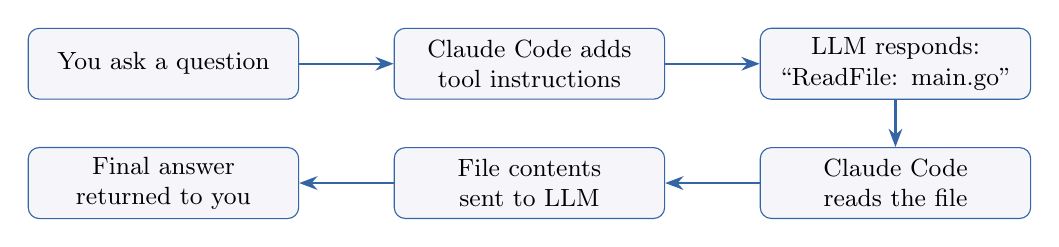
\begin{tikzpicture}[
  node distance=0.6cm and 1.2cm,
  box/.style={rectangle, rounded corners, draw=popblue, fill=lightbg,
              text width=3.2cm, minimum height=0.9cm, align=center,
              font=\small},
  arr/.style={-Stealth, thick, popblue}
]
  \node[box] (user) {You ask a question};
  \node[box, right=of user] (cc) {Claude Code adds\\tool instructions};
  \node[box, right=of cc] (llm) {LLM responds:\\``ReadFile: main.go''};
  \node[box, below=of llm] (exec) {Claude Code\\reads the file};
  \node[box, left=of exec] (back) {File contents\\sent to LLM};
  \node[box, left=of back] (ans) {Final answer\\returned to you};
  \draw[arr] (user) -- (cc);
  \draw[arr] (cc) -- (llm);
  \draw[arr] (llm) -- (exec);
  \draw[arr] (exec) -- (back);
  \draw[arr] (back) -- (ans);
\end{tikzpicture}
\end{center}

\bigskip
\begin{block}{Why Claude's tool use matters}
Strong tool use $\Rightarrow$ tackles harder tasks, extensible platform, better security (no full-codebase indexing).
\end{block}
\end{frame}

% ══════════════════════════════════════════════
% SECTION 2: Getting Hands On
% ══════════════════════════════════════════════
\section{Getting Hands On}

\begin{frame}[fragile]{Setup \& Project Initialization}
\textbf{Installation:}
\begin{lstlisting}[language=bash]
claude install          # recommended
# or: npm install -g @anthropic-ai/claude-code
cd your-project
claude          # launches Claude Code
\end{lstlisting}

\bigskip
\textbf{The \texttt{/init} command:}
\begin{itemize}
  \item Analyzes your entire codebase
  \item Creates a \texttt{CLAUDE.md} summary (architecture, commands, patterns)
  \item Included in \emph{every} request --- persistent system prompt
\end{itemize}

\bigskip
\begin{alertblock}{Tip}
Press \textbf{Shift+Tab} to cycle permission modes (e.g.\ auto-accept edits for the session).
\end{alertblock}
\end{frame}

% ──────────────────────────────────────────────
\begin{frame}[fragile]{Adding Context: CLAUDE.md}
\textbf{Three locations, three scopes:}
\begin{table}
\centering\small
\begin{tabular}{lll}
\textbf{File} & \textbf{Scope} & \textbf{Shared?} \\
\hline
\texttt{CLAUDE.md} & Project & Yes (committed) \\
\texttt{CLAUDE.local.md} & Project & No (personal) \\
\texttt{\textasciitilde/.claude/CLAUDE.md} & All projects & No (global) \\
\end{tabular}
\end{table}

\bigskip
\textbf{Memory mode with \texttt{\#}:}
\begin{lstlisting}
# Use comments sparingly. Only comment complex code.
\end{lstlisting}
Claude merges this instruction into your \texttt{CLAUDE.md} automatically.

\bigskip
\textbf{File mentions with \texttt{@}:}
\begin{lstlisting}
How does the auth system work? @auth
\end{lstlisting}
Includes the file's contents in the request. Also works inside \texttt{CLAUDE.md}.
\end{frame}

% ──────────────────────────────────────────────
\begin{frame}{Making Changes}
\textbf{Key techniques:}
\begin{itemize}
  \item \textbf{Screenshots} --- paste images directly; Claude reads error messages, UI issues
  \item \textbf{Planning mode} --- one of the \texttt{Shift+Tab} modes; Claude outlines steps before executing
  \item \textbf{Adaptive thinking} --- Claude adjusts reasoning depth; tune with \texttt{/effort}
  \item \textbf{Auto mode} --- classifier auto-approves safe operations, blocks risky ones
\end{itemize}

\bigskip
\begin{exampleblock}{Workflow}
\begin{enumerate}
  \item Describe the problem or feature
  \item Let Claude explore, plan, and implement
  \item Review the diff, approve or redirect
\end{enumerate}
\end{exampleblock}
\end{frame}

% ──────────────────────────────────────────────
\begin{frame}{Controlling Context}
\begin{columns}[T]
\column{0.5\textwidth}
\textbf{\color{popblue}Interrupt \& Redirect}
\begin{itemize}
  \item \textbf{Escape} --- stop mid-response, redirect
  \item \textbf{Escape $\times$ 2} --- rewind to earlier point
  \item Combine with \texttt{\#} to fix repeating errors
\end{itemize}

\column{0.5\textwidth}
\textbf{\color{paramgreen}Commands}
\begin{itemize}
  \item \texttt{/compact} --- summarize history, keep knowledge
  \item \texttt{/clear} --- fresh start, no prior context
  \item Auto-compaction at $\sim$95\% context capacity
\end{itemize}
\end{columns}

\bigskip
\begin{alertblock}{When to use what}
\texttt{/compact} when switching to a \emph{related} task (preserves context). \\
\texttt{/clear} when switching to an \emph{unrelated} task (avoids confusion).
\end{alertblock}
\end{frame}

% ──────────────────────────────────────────────
\begin{frame}[fragile]{Custom Commands}
\textbf{Create reusable commands:}
\begin{enumerate}
  \item Create \texttt{.claude/commands/audit.md}
  \item Filename becomes the command: \texttt{/audit}
  \item Restart Claude Code
\end{enumerate}

\bigskip
\textbf{Commands with arguments (\texttt{\$ARGUMENTS}):}
\begin{lstlisting}
Write comprehensive tests for: $ARGUMENTS

Testing conventions:
* Use Vitest with React Testing Library
* Place test files in __tests__/ next to source
* Name test files as [filename].test.ts(x)

Coverage: happy paths, edge cases, error states
\end{lstlisting}

\textbf{Usage:}
\begin{lstlisting}
/write_tests the use-auth.ts file in the hooks directory
\end{lstlisting}
\end{frame}

% ──────────────────────────────────────────────
\begin{frame}[fragile]{MCP Servers}
\textbf{Model Context Protocol} --- extend Claude with new tools.

\bigskip
\textbf{Example: Playwright (browser control)}
\begin{lstlisting}[language=bash]
claude mcp add playwright npx @playwright/mcp@latest
\end{lstlisting}

\textbf{Pre-approve permissions} in \texttt{.claude/settings.local.json}:
\begin{lstlisting}[]
{
  "permissions": {
    "allow": ["mcp__playwright"],
    "deny": []
  }
}
\end{lstlisting}

\bigskip
\textbf{Ecosystem:} database interactions, API testing, cloud integrations, file operations, dev tool automation\ldots

\textbf{Deferred loading:} MCP tools lazy-load via \texttt{ToolSearch}, cutting context usage up to 95\%.
\end{frame}

% ──────────────────────────────────────────────
\begin{frame}{GitHub Integration}
Run \texttt{/install-github-app} in Claude Code.

\bigskip
\textbf{Two workflows added to \texttt{.github/workflows/}:}
\begin{enumerate}
  \item \textbf{Mention Action} --- \texttt{@claude} in issues/PRs $\to$ Claude analyzes \& responds
  \item \textbf{PR Review Action} --- auto-reviews every pull request
\end{enumerate}

\bigskip
\textbf{Customization options:}
\begin{itemize}
  \item \texttt{custom\_instructions:} --- project-specific context
  \item \texttt{mcp\_config:} --- attach MCP servers (e.g.\ Playwright)
  \item \texttt{allowed\_tools:} --- explicit tool permissions (required in CI)
\end{itemize}
\end{frame}

% ══════════════════════════════════════════════
% SECTION 3: Hooks & SDK
% ══════════════════════════════════════════════
\section{Hooks \& SDK}

\begin{frame}{Hooks: Architecture}
\begin{center}
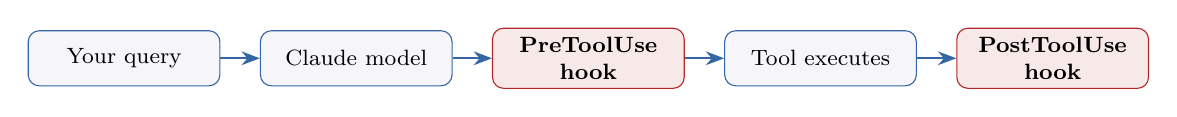
\begin{tikzpicture}[
  node distance=0.4cm and 0.5cm,
  box/.style={rectangle, rounded corners, draw=popblue, fill=lightbg,
              text width=2.2cm, minimum height=0.7cm, align=center, font=\footnotesize},
  hook/.style={rectangle, rounded corners, draw=warnred, fill=warnred!10,
               text width=2.2cm, minimum height=0.7cm, align=center, font=\footnotesize\bfseries},
  arr/.style={-Stealth, thick, popblue}
]
  \node[box] (query) {Your query};
  \node[box, right=of query] (llm) {Claude model};
  \node[hook, right=of llm] (pre) {PreToolUse\\hook};
  \node[box, right=of pre] (tool) {Tool executes};
  \node[hook, right=of tool] (post) {PostToolUse\\hook};
  \draw[arr] (query) -- (llm);
  \draw[arr] (llm) -- (pre);
  \draw[arr] (pre) -- (tool);
  \draw[arr] (tool) -- (post);
\end{tikzpicture}
\end{center}

\begin{columns}[T]
\column{0.5\textwidth}
\textbf{\color{warnred}PreToolUse}
\begin{itemize}
  \item Runs \emph{before} tool call
  \item Can \textbf{block or rewrite} the operation
  \item Access control, validation
\end{itemize}

\column{0.5\textwidth}
\textbf{\color{paramgreen}PostToolUse}
\begin{itemize}
  \item Runs \emph{after} tool call
  \item Cannot block (already done)
  \item Formatting, testing, logging
\end{itemize}
\end{columns}

\bigskip
\small
\textbf{Hook types:} \texttt{"command"} (shell) $|$ \texttt{"http"} (POST JSON to URL)\\
\textbf{Config locations:} \texttt{\textasciitilde/.claude/settings.json} (global) $|$
\texttt{.claude/settings.json} (team) $|$
\texttt{.claude/settings.local.json} (personal)
\end{frame}

% ──────────────────────────────────────────────
\begin{frame}[fragile]{Hook Configuration}
\textbf{PreToolUse example} --- guard specific tool calls:
\begin{lstlisting}[]
"PreToolUse": [{
  "matcher": "Read|Grep",
  "hooks": [{
    "type": "command",
    "command": "node ./hooks/read_hook.js"
  }]
}]
\end{lstlisting}
\smallskip
\textbf{PostToolUse example} --- run formatter after edits:
\begin{lstlisting}[]
"PostToolUse": [{
  "matcher": "Write|Edit|MultiEdit",
  "hooks": [{
    "type": "command",
    "command": "node ./hooks/format_hook.js"
  }]
}]
\end{lstlisting}
\end{frame}

% ──────────────────────────────────────────────
\begin{frame}[fragile]{Implementing a Hook: Protect \texttt{.env}}
\begin{lstlisting}[]
async function main() {
  const chunks = [];
  for await (const chunk of process.stdin) {
    chunks.push(chunk);
  }
  const toolArgs = JSON.parse(
    Buffer.concat(chunks).toString()
  );

  const readPath =
    toolArgs.tool_input?.file_path
    || toolArgs.tool_input?.path || "";

  if (readPath.includes('.env')) {
    console.error("You cannot read the .env file");
    process.exit(2);  // exit code 2 = block
  }
}

main();
\end{lstlisting}

\small
Hook receives tool call data via \texttt{stdin} as JSON. Exit code \texttt{2} blocks the operation with an error message back to Claude.
\end{frame}

% ──────────────────────────────────────────────
\begin{frame}{Hook Gotchas \& Practical Recipes}
\begin{alertblock}{Common Gotchas}
\begin{itemize}\setlength\itemsep{0em}
  \item Use \textbf{absolute paths} in hook commands
  \item Restart Claude Code after changing hooks
  \item Test hooks with simple cases first
\end{itemize}
\end{alertblock}

\smallskip
\small
\textbf{Useful hook ideas:}
\begin{itemize}\setlength\itemsep{0em}
  \item \textbf{TypeScript type-checking} --- run \texttt{tsc} after edits, feed errors back
  \item \textbf{Auto-formatting} --- run Prettier/Black after writes
  \item \textbf{Query duplication prevention} --- detect duplicate SQL/API calls
  \item \textbf{Test runner} --- auto-run tests on changed files
  \item \textbf{Sensitive file protection} --- block access to credentials
\end{itemize}

\smallskip
\footnotesize
\textbf{Other hook events:} Notification, Stop, SubagentStop, PreCompact, UserPromptSubmit, SessionStart, SessionEnd.
\end{frame}

% ──────────────────────────────────────────────
\begin{frame}[fragile]{The Claude Code SDK}
\textbf{Claude Agent SDK} --- run Claude Code programmatically (TypeScript, Python, CLI).

\begin{lstlisting}[]
import { query } from "@anthropic-ai/claude-code";

const prompt = "Look for duplicate queries in ./src/queries";

for await (const message of query({ prompt })) {
  console.log(JSON.stringify(message, null, 2));
}
\end{lstlisting}

\textbf{Permissions:} read-only by default. Enable writes with:
\begin{lstlisting}[]
for await (const message of query({
  prompt,
  options: { allowedTools: ["Edit"] }
})) { /* ... */ }
\end{lstlisting}

\smallskip
\textbf{Use cases:} Git hooks for code review, CI/CD quality checks, automated documentation, build optimization scripts.
\end{frame}

% ──────────────────────────────────────────────
\begin{frame}{Summary}
\begin{columns}[T]
\column{0.5\textwidth}
\begin{block}{Core Concepts}
\begin{itemize}
  \item Tool use makes LLMs practical
  \item \texttt{CLAUDE.md} = persistent context
  \item \texttt{@} mentions for file focus
  \item \texttt{/compact} vs \texttt{/clear}
\end{itemize}
\end{block}

\column{0.5\textwidth}
\begin{block}{Power Features}
\begin{itemize}
  \item Custom commands (\texttt{\$ARGUMENTS})
  \item MCP servers (deferred tool loading)
  \item Hooks (block, rewrite, HTTP)
  \item Claude Agent SDK
  \item Auto mode, adaptive thinking
  \item Voice (\texttt{/voice}), remote control
\end{itemize}
\end{block}
\end{columns}

\vfill
\centering
\Large\color{popblue} Questions?
\end{frame}

\end{document}
